% =====================================================================================
% REVISIÓN 3  -  PROYECTOS DE INVESTIGACIÓN (algoritmo, modelo de aprendizaje de máquina u otro)
% Para usarla pon \TipoProyecto{investigacion} en configuracion/datos.tex, activa esta línea en main.tex
% y comenta la de secciones/06_desarrollo_sistema.
% Escribe tu texto FUERA de los recuadros \begin{guia} ... \end{guia}.
% =====================================================================================

\section{Experimentación} \label{sec:experimentacion}

\begin{guia}[Guía: Experimentación (Revisión 3, proyectos de investigación)]
Este capítulo tiene tres partes: \emph{Diseño de experimentos}, \emph{Resultados experimentales} y
\emph{Conclusiones de los resultados experimentales}. Las tres deben ser coherentes con tu hipótesis, tus objetivos y
la propuesta de solución. Todas las figuras y tablas llevan \verb|\caption|, \verb|\label| y se citan con
\verb|\ref| (nunca ``Figura 3'' escrito a mano).
\end{guia}

\subsection{Diseño de experimentos} \label{sec:diseno_experimentos} % audit:req=diseno_experimentos

\begin{guia}[Guía: Diseño de experimentos (estadístico y con metodología de experimentación)]
\textbf{¿Para qué sirve?} Define, antes de mostrar resultados, cómo vas a probar tu hipótesis de forma que otra persona
pueda repetirlo.

\textbf{Debe responder:}
\begin{itemize}[nosep,leftmargin=*]
  \item ¿Cuál es la hipótesis y su formulación estadística (hipótesis nula $H_0$ y alternativa $H_1$)?
  \item ¿Cuáles son las variables independientes (factores y niveles) y dependientes (métricas de desempeño)? ¿por qué
        esas métricas?
  \item ¿Qué diseño experimental usas (factorial, completamente aleatorizado, por bloques, validación cruzada de $k$
        pliegues, etc.) y por qué es adecuado?
  \item ¿Qué datos usas (origen, tamaño, preprocesamiento, partición entrenamiento/validación/prueba) y cómo evitas
        fugas de información?
  \item ¿Con qué líneas base o métodos del estado del arte comparas?
  \item ¿Cuántas repeticiones o semillas ejecutas y por qué son suficientes?
  \item ¿Qué prueba estadística usarás (t de Student, ANOVA, Wilcoxon, Friedman\ldots), con qué nivel de significancia, y
        qué supuestos verificas?
  \item ¿Cómo garantizas la reproducibilidad (versiones, hardware, semillas, hiperparámetros, repositorio de código)?
\end{itemize}

\textbf{Extensión mínima:} 250 palabras. Resume los parámetros en una tabla.

\textbf{Errores frecuentes:} una sola ejecución sin repeticiones; comparar contra una línea base débil; evaluar en los
mismos datos de entrenamiento; no justificar las métricas; no declarar hiperparámetros.

\textbf{Cómo se revisa:} validez estadística, comparabilidad y reproducibilidad.
\end{guia}

% >>> ESCRIBE AQUÍ el diseño de experimentos <<<


\subsubsection{Hipótesis de investigación}

La investigación busca determinar si los modelos de lenguaje de 1-bit presentan diferencias en la calidad de sus respuestas y en los recursos computacionales necesarios para ejecutarlos.

Hipótesis nula ($H_0$): No existen diferencias entre los modelos evaluados en los parámetros de desempeño comparables bajo condiciones experimentales equivalentes.

Hipótesis alternativa ($H_1$): Al menos dos modelos presentan diferencias en uno o más de esos parámetros.

Para cada métrica susceptible de análisis estadístico, se establece:

\[
H_0:\theta_1=\theta_2=\cdots=\theta_k
\]

\[
H_1:\exists\,i\neq j\text{ tal que }\theta_i\neq\theta_j
\]

Donde $\theta$ representa el parámetro de la métrica analizada y $k$ el número de modelos comparados. El contraste se realiza por métrica, sin suponer de antemano la superioridad de una implementación.

\subsubsection{Variables independientes y dependientes}

El factor principal es el modelo de lenguaje de 1-bit, cuyos niveles corresponden a las implementaciones seleccionadas. Se documentan además la representación de los pesos y la configuración de inferencia, pues influyen en el rendimiento observado.

La evaluación considera diez métricas:

\begin{enumerate}[nosep,leftmargin=*,itemsep=1pt]
\item Perplejidad: capacidad para predecir secuencias de texto.
\item Exactitud: proporción de respuestas correctas.
\item Tamaño: espacio ocupado por el archivo del modelo.
\item Memoria: memoria utilizada durante la ejecución.
\item Latencia: tiempo empleado para generar una respuesta.
\item Velocidad: tokens generados por segundo.
\item Energía: consumo energético de la ejecución.
\item Bits por peso: precisión de representación de los parámetros.
\item Compresión: reducción del tamaño frente a una referencia.
\item Pérdida: error de predicción según una función definida.
\end{enumerate}

La exactitud, la perplejidad y la pérdida caracterizan la calidad de las predicciones; memoria, latencia, velocidad y energía describen el desempeño de ejecución; tamaño, bits por peso y compresión son indicadores de almacenamiento y representación. Estas métricas permiten estudiar tanto la calidad de las respuestas como la viabilidad técnica.

\subsubsection{Diseño experimental}

Se emplea un diseño comparativo por bloques, donde cada pregunta del conjunto de evaluación constituye un bloque. Los modelos reciben los mismos enunciados y opciones, y sus respuestas se contrastan con la clave correspondiente.

El procedimiento comprende preparar la implementación, ejecutar las preguntas, evaluar las respuestas y organizar los registros en archivos CSV. Este diseño permite comparar la exactitud sobre unidades comunes. Para las métricas computacionales se consideran también las diferencias de configuración y formato de los modelos, que pueden afectar las mediciones.

\subsubsection{Datos utilizados}

Se utiliza el conjunto \textit{ARC (AI2 Reasoning Challenge)}, configuración \textit{ARC-Easy}, disponible en Hugging Face. Su partición de prueba contiene 2,376 preguntas de ciencias de opción múltiple, con identificadores, alternativas y respuestas correctas.

Las preguntas se presentan mediante un formato común que conserva su contenido y opciones. Las respuestas generadas se identifican y normalizan para compararlas con la clave de cada registro. Las consultas, respuestas y métricas se organizan en archivos CSV.

Los modelos son previamente desarrollados y no se entrenan ni ajustan con las respuestas de prueba. No se realiza una partición propia de entrenamiento y validación. Aunque así se evita utilizar la clave de prueba durante un entrenamiento propio, no es posible descartar coincidencias con los datos originales de preentrenamiento.

\subsubsection{Líneas base y métodos del Estado del arte}

La comparación experimental utiliza como referencia las respuestas correctas de ARC-Easy y los resultados de los modelos ante las mismas preguntas. La clave del dataset sirve para determinar aciertos, pero no constituye por sí misma un modelo de línea base.

Como referencias del Estado del arte se consideran BitNet, basado en entrenamiento con pesos de baja precisión \cite{bitnetJMLR2025}; PT-BitNet, que aplica cuantización posterior al entrenamiento \cite{ptBitnet2025}; y el estudio comparativo de técnicas de compresión en distintas plataformas realizado por Hildebrand y colaboradores \cite{compressionComparison2026}. Estos trabajos permiten contrastar enfoques de representación y criterios de eficiencia.

Los valores publicados se utilizan como contexto técnico y no como mediciones directamente equivalentes cuando difieren los modelos, datos, equipos o procedimientos. No se declara una línea base propia de precisión completa si no se dispone de su ejecución comparable.

\subsubsection{Repeticiones y semillas}

El procedimiento establece una respuesta evaluable por pregunta y configuración del modelo. ARC-Easy proporciona 2,376 preguntas en su partición de prueba; este número corresponde al tamaño del conjunto, no a 2,376 repeticiones de una misma ejecución.

Una respuesta por pregunta permite calcular la exactitud sobre los reactivos efectivamente procesados, pero no basta para estimar la estabilidad de las respuestas ni la variabilidad entre ejecuciones. Los registros revisados no acreditan un número uniforme de repeticiones ni semillas fijas para todas las implementaciones. Por tanto, no se considera demostrada la suficiencia de repeticiones para las métricas computacionales; sus resultados se reportan con el alcance que permiten los registros disponibles.

\subsubsection{Pruebas estadísticas}

Se adopta un nivel de significancia de $\alpha=0.05$. Para contrastar diferencias de exactitud entre tres o más modelos evaluados sobre las mismas preguntas, se utilizará la prueba Q de Cochran, a partir de resultados binarios (correcto o incorrecto). Para comparaciones entre pares se utilizará la prueba exacta de McNemar, con ajuste de Holm si se realizan múltiples contrastes.

Se verificará que las implementaciones hayan respondido los mismos reactivos, que cada resultado pueda clasificarse de forma binaria y que las preguntas constituyan unidades de evaluación independientes para el contraste. Si no se dispone de registros completos y pareados, no se aplicará la prueba correspondiente.

Las métricas continuas se resumirán mediante valores y medidas de dispersión. Si existen mediciones pareadas suficientes y condiciones de ejecución comparables, se empleará Friedman para varios modelos o Wilcoxon de rangos con signo para comparaciones por pares, verificando los supuestos de cada prueba. Los valores $p$ se reportarán únicamente después de calcularse sobre datos reales.

\subsubsection{Reproducibilidad}

Las pruebas se desarrollan en un emulador Android 17 (API 37), arquitectura x86\_64, preparado con Android Studio, SDK, NDK y ADB. La ejecución se realiza desde terminal mediante herramientas basadas en \texttt{llama.cpp} y archivos GGUF cuando son compatibles. El conjunto de evaluación corresponde a ARC-Easy, partición \textit{test}, disponible en \url{https://huggingface.co/datasets/allenai/ai2_arc}.

Los archivos CSV organizan las consultas, las respuestas y las métricas; las evidencias de ejecución permiten revisar el procedimiento. El repositorio \url{https://github.com/MarceloZR/Plantilla-Tesina-ITI} contiene la documentación de la tesina, por lo que no se presenta como repositorio del código ejecutable de las pruebas.

Para reproducir exactamente cada ejecución deben identificarse el equipo anfitrión, las versiones de software, el archivo y formato de pesos, los parámetros de generación y las semillas. La documentación revisada no acredita todos esos datos para cada implementación; esta carencia limita la repetición exacta del experimento y se declara expresamente, sin asignar configuraciones no verificadas.

\subsubsection{Parámetros experimentales}

La Tabla~\ref{tab:parametros_experimentales} resume las condiciones principales del diseño.

\begin{table}[H]
\centering
\small
\caption{Parámetros del diseño experimental.}
\label{tab:parametros_experimentales}
\begin{tabular}{L{4.1cm}L{10.4cm}}
\toprule
Parámetro & Descripción \\
\midrule
Tipo y diseño & Estudio comparativo por bloques de preguntas \\
Factor principal & Modelo e implementación de lenguaje de 1-bit \\
Conjunto de evaluación & ARC (AI2 Reasoning Challenge), ARC-Easy \\
Partición y tamaño & Prueba (\textit{test}), 2,376 preguntas de opción múltiple \\
Criterio de exactitud & Coincidencia con la respuesta correcta del dataset \\
Entorno & Android 17, API 37, x86\_64 \\
Herramientas & Android Studio, SDK, NDK, ADB y llama.cpp \\
Modelos & Archivos GGUF cuando sean compatibles \\
Métricas & Perplejidad, exactitud, tamaño, memoria, latencia, velocidad, energía, bits por peso, compresión y pérdida \\
Registro & Archivos CSV y evidencias de ejecución \\
Contraste de exactitud & Q de Cochran; McNemar exacta en comparaciones por pares \\
Nivel de significancia & $\alpha=0.05$ \\
Repeticiones & Una respuesta por reactivo y configuración; no equivale a réplicas \\
Semillas & Sin registro uniforme acreditado para todas las implementaciones \\
\bottomrule
\end{tabular}
\end{table}


\subsection{Resultados experimentales} \label{sec:resultados_experimentales} % audit:req=resultados_experimentales

\begin{guia}[Guía: Resultados experimentales]
\textbf{¿Para qué sirve?} Presenta lo que se obtuvo, con objetividad y sin interpretar todavía.

\textbf{Debe responder:}
\begin{itemize}[nosep,leftmargin=*]
  \item ¿Qué resultados se obtuvieron para cada experimento y cada objetivo específico? Preséntalos en tablas y gráficas
        (media $\pm$ desviación estándar, intervalos de confianza).
  \item ¿Cómo se comparan contra las líneas base? ¿las diferencias son estadísticamente significativas (reporta el
        valor $p$ o el estadístico)?
  \item ¿Hubo resultados negativos, inesperados o atípicos? Repórtalos también.
\end{itemize}

\textbf{Extensión mínima:} 200 palabras, además de las tablas y figuras. Cada tabla o figura se cita y se describe en
el texto.

\textbf{Errores frecuentes:} mostrar solo el mejor caso; gráficas sin ejes ni unidades; tablas sin comentarios; omitir la
variabilidad.

\textbf{Cómo se revisa:} que los resultados respondan al diseño planteado y se presenten con rigor.
\end{guia}

% >>> ESCRIBE AQUÍ los resultados experimentales <<<

\subsubsection{Resultados obtenidos}

Las primeras evaluaciones se realizaron mediante diez preguntas elaboradas manualmente, relacionadas con matemáticas, vocabulario, conocimientos generales y seguimiento de instrucciones. En las dos implementaciones con resultados documentados se registraron 10 aciertos de 10 consultas y 0 aciertos de 10, respectivamente. La Tabla~\ref{tab:resultados_62} reúne los valores obtenidos de las diez métricas seleccionadas para la investigación.

\begin{table}[H]
\centering
\footnotesize
\renewcommand{\arraystretch}{1.10}
\caption{Resultados de las evaluaciones iniciales.}
\label{tab:resultados_62}
\begin{tabular}{L{2.60cm}L{5.65cm}L{5.10cm}}
\toprule
Métrica & BitNet b1.58 (I2\_S) & FBI-LLM 130M (F32) \\
\midrule
Perplejidad & - & 29.9849 \\
Exactitud & 100\,\% (10/10) & 0\,\% (0/10) \\
Tamaño & - & 512.27 MiB \\
Memoria & 1,212.54 MiB & 569.49 MiB \\
Latencia & - & 0.36 s/respuesta \\
Velocidad & 6.64--10.10 tokens/s & 70.94 tokens/s \\
Energía & - & 105.957 J (estimado) \\
Bits por peso & 1.58 teóricos; archivo I2\_S & 32 bits; archivo F32 \\
Compresión & 90.1\,\% teórica frente a FP16 & 1.00 veces respecto al original \\
Pérdida & - & 3.4007 \\
\bottomrule
\end{tabular}
\end{table}

En estas primeras pruebas, la configuración con mayor exactitud registró un consumo de memoria más elevado y una menor velocidad de generación, mientras que la otra utilizó menos memoria y produjo texto más rápidamente. La Figura~\ref{fig:memoria_62} permite visualizar la diferencia de memoria, teniendo en cuenta que las configuraciones emplearon representaciones de pesos distintas.

\begin{figure}[H]
\centering
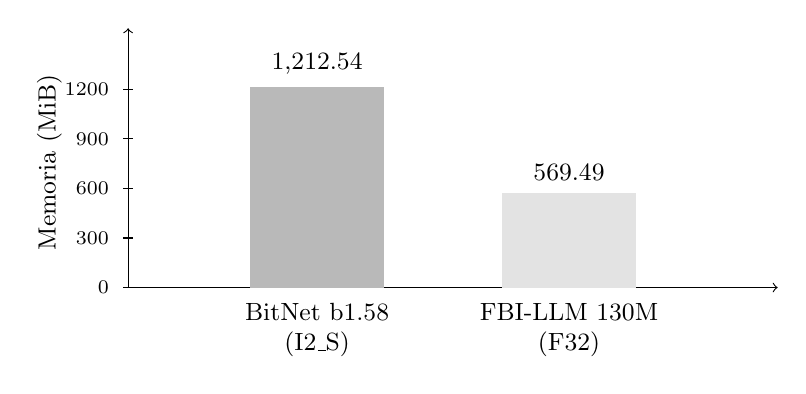
\begin{tikzpicture}[x=1cm,y=0.74cm]
\draw[->] (0,0)--(0,4.45);
\draw[->] (0,0)--(8.25,0);
\foreach \v/\y in {0/0,300/0.85,600/1.70,900/2.55,1200/3.40}{
\draw (-0.06,\y)--(0.06,\y);
\node[left,font=\scriptsize] at (-0.12,\y){\v};
}
\node[rotate=90,font=\small] at (-1.00,2.15){Memoria (MiB)};
\fill[gray!55] (1.55,0) rectangle (3.25,3.4355);
\fill[gray!22] (4.75,0) rectangle (6.45,1.6136);
\node[above,font=\small] at (2.40,3.49){1,212.54};
\node[above,font=\small] at (5.60,1.67){569.49};
\node[below,align=center,font=\small] at (2.40,-0.10){BitNet b1.58\\(I2\_S)};
\node[below,align=center,font=\small] at (5.60,-0.10){FBI-LLM 130M\\(F32)};
\end{tikzpicture}
\caption{Memoria registrada durante las primeras evaluaciones.}
\label{fig:memoria_62}
\end{figure}

\filbreak
\subsubsection{Comparación con las líneas base y análisis estadístico}

En las diez preguntas iniciales, BitNet b1.58 obtuvo 10 aciertos (100\,\%) y FBI-LLM 130M no obtuvo respuestas correctas (0\,\%). En cambio, la segunda implementación registró menor uso de memoria (569.49 frente a 1,212.54 MiB) y mayor velocidad (70.94 frente a 6.64--10.10 tokens/s). Los resultados muestran diferencias entre exactitud y rendimiento, pero no permiten determinar qué modelo es mejor en todas las condiciones, porque se ejecutaron con configuraciones y formatos de pesos distintos.

El contraste exacto de McNemar para los aciertos de las mismas diez consultas produjo $p=0.001953125$. Los intervalos de confianza de Wilson al 95\,\% fueron de 72.25--100\,\% y de 0--27.75\,\%, respectivamente. Estas cifras corresponden únicamente a las preguntas iniciales y no a ARC-Easy. No se dispuso de una línea base de precisión completa ejecutada en condiciones equivalentes ni de suficientes repeticiones para calcular la media $\pm$ desviación estándar de memoria y velocidad.

\subsubsection{Resultados negativos, errores y cambio de metodología}

Durante las primeras pruebas se registraron respuestas incorrectas, repeticiones de texto y salidas incompletas por el límite de 24 tokens. Algunas implementaciones también presentaron dificultades de compatibilidad durante su ejecución.

Reconocí tres errores principales en el procedimiento inicial: utilicé solo diez preguntas manuales, no organicé los resultados en archivos CSV desde el comienzo y no establecí una forma consistente de obtener las diez métricas. Por ello, varias mediciones quedaron sin obtener y se representan con un guion (-) en la Tabla~\ref{tab:resultados_62}; esto no significa que su valor fuera cero.

Para corregir estos errores cambié la metodología de trabajo. Incorporé ARC-Easy, con 2,376 preguntas en su partición de prueba, y organicé los registros en archivos CSV para relacionar consultas, respuestas y métricas. Las pruebas iniciales se conservaron como evidencia de los resultados obtenidos y de las dificultades encontradas. No se presentan aquí resultados estadísticos de ARC-Easy porque los registros disponibles todavía no permiten verificarlos.


\subsection{Conclusiones de los resultados experimentales} \label{sec:conclusiones_resultados} % audit:req=conclusiones_resultados

\begin{guia}[Guía: Conclusiones de los resultados experimentales]
\textbf{Debe responder:} ¿qué dicen los resultados sobre la hipótesis (se acepta, se rechaza o se sustenta parcialmente) y
con qué evidencia (cita la tabla o figura)? ¿qué objetivos específicos se cumplieron? ¿qué amenazas a la validez hay
(datos, métricas, supuestos)? ¿qué sorprendió?

\textbf{Mínimo:} 60 palabras. No afirmes más de lo que los resultados sustentan. Las conclusiones generales del proyecto
van en el capítulo \emph{Conclusiones} (Revisión 4).
\end{guia}

% >>> ESCRIBE AQUÍ las conclusiones de los resultados experimentales <<<
